\section{INTRODUCTION} \label{sec:introduction}
    \IEEEPARstart{M}{ost} \acrlong{ML} or \gls{NN} based methods, rely upon a workflow where a model is designed, trained, validated, and deployed~\cite{Krose2011AnNetworks}. %This is logical as the intention with \gls{NN} based methods is to treat them as a general function approximator~\cite{Krose2011AnNetworks}. This is where the function is determined by the relationship between the data used and the objective or loss function. 
    However, in the domain of image denoising, the \gls{DIP} method has received attention as training and inference are performed independently on each new image~\cite{Ulyanov2018DeepPrior}. %The \gls{DIP} method could be considered to be a custom learnt bank of filters for each input. In order to prevent overfitting, the number of iterations used is imperative.% The authors of the original \gls{DIP} paper argue that the method could be considered to be used to solve many inverse problems~\cite{Ulyanov2018DeepPrior}.
    
    For \acrshort{PET}, there have been a number of adaptations of \gls{DIP}.~\cite{Gong2019PETPrior} used a U-Net with relatively high count/low motion brain scans~\cite{Weng2015U-Net:Segmentation}. In~\cite{Hashimoto20214DNetwork} \gls{DIP} is extended to \acrshort{4D} dynamic \acrshort{PET}. To do this, multiple output branches are grafted onto the \gls{NN}, one for each dynamic time point.~\cite{Hashimoto2019DynamicDatasets} uses the original or static \acrshort{PET} acquisition as input to the \gls{NN}, rather than noise.~\cite{Yang2022SimultaneousPrior} represents a more recent extension, where multiple \glss{NN} are used simultaneously.
    
    This work seeks to extend or simplify previous work, in order to denoise \acrshort{4D} dynamic \acrshort{PET} data.

% \vspace{-0.4cm}
    
\section{METHODS}\label{sec:methods}
    \subsection{Network Design and Execution} \label{sec:network_design_and_execution}
        Firstly, we reduced \acrshort{GPU} memory requirements. Because \gls{DIP} requires training at inference, the full amount of memory is needed every time the method is used. To aid in clinical adoption, a hard limit of \SI{8.0}{\giga\byte} \acrshort{GPU} memory was imposed. Secondly, a more robust stopping criteria is required. %The stopping criteria should be flexible so as to allow the method to correct a wider variety of inputs. 
        % One method would be, to look at a window of previous loss function values, and exit, when the gradient of this drops below a tolerance.
        To aid in achieving this, as well as to address weaknesses of the original \gls{DIP}, regularisation must be added, so as to stop the \gls{NN} fitting to noise, similar to~\cite{Liu2019ImagePrior}. Finally, because the output from this method is to be used in a further kinetic model fitting, it may provide improved results to have a metric of the uncertainty in the denoised images. we used dropout as in~\cite{Gal2015DropoutLearning} to approximate (more expensive) Bayesian inference. Furthermore, this work uses \acrshort{PET} data with a \gls{FOV} of the lung and liver, whereas most previous work uses a \gls{FOV} of the head.
    
        The \gls{NN} used was a modified U-Net~\cite{Weng2015U-Net:Segmentation}, with seven down/upsampling stages. Each down/upsampling stage consisted of two convolutional layers (with two, four, eight, $16$, $32$, $64$, or $128$ channels, depending on depth). Followed by, either a split strided convolution and maxpooling layer (with the result concatenated), or a trilinear upsampling layer. Edge padding, group normalisation~\cite{Wu2018GroupNormalization}, MISH activation~\cite{Misra2020Mish:Function}, and spatial dropout, were used with every convolutional layer. Data was edge padded to the nearest power of two, and the input data had Gaussian noise summed to it. Both input and label data were standardised. \acrlong{MSE} and \gls{TV} were used as the loss function. AdamW~\cite{Loshchilov2017DecoupledRegularization} was used as optimiser. Training continued for all methods until the gradient of the loss function, over a window of previous results, reduced below a threshold. Parameters were tuned using a grid search.
        
        Two training regimes were explored, one where each time point was treated independently, and another, where the model weights were saved and then independently updated on each time point (the mean of the new models weights was taken for the next iteration).
        
    % \vspace{-0.4cm}
    
    \subsection{\acrshort{PET} Acquisition Simulation and Image Reconstruction} \label{sec:pet_acquisition_simulation_and_image_reconstruction}
        A series of dynamic scans, following the clinical \acrlong{DWB}-\acrshort{PET} protocol, were generated using the \acrshort{XCAT} phantom~\cite{segars4DXCATPhantom2010}. Patient-derived kinetic parameters were assigned to; $64$ tissues, three tumours of \SI{1.0}{\centi\meter} diameter in the left lung, and three tumours of \SI{2.5}{\centi\meter}, \SI{2.0}{\centi\meter} and \SI{1.0}{\centi\meter} diameter in the liver. An input function for \acrshort{18F-FDG}, taken from~\cite{langsjoEffectsSubanestheticKetamine2004}, was used to simulate \glss{TAC} to create dynamic images.
% KT some info here on timing

        \acrshort{PET} acquisitions were simulated (and reconstructed) using \acrshort{STIR}~\cite{Thielemans2012} through \acrshort{SIRF}~\cite{Ovtchinnikov2017}. \acrlong{NTOF} sinogram data were simulated, using resolution modelling (using a \SI{6.0}{\centi\meter} \acrshort{FWHM} Gaussian filter). Randoms and scatter were not included. Poisson noise was added.% corresponding to a total number of counts of XXX in time frame XXX.
% KT some info above

        Finally, all data sets were reconstructed using $10$ iterations with $17$ subsets of \acrshort{OSEM}~\cite{Hudson1994}.

    % \vspace{-0.4cm}
    
    \subsection{Kinetic Modelling} \label{sec:kinetic_modelling}
        Indirect Patlak estimation was used to generate $K_i$ and intercept images~\cite{patlak1983GraphicalEvaluationBloodtoBrain}. \glss{VOI} were defined for the three lesions and two background regions (lung and liver), and the mean values of $K_i$ and $V_d$ were calculated in each \gls{VOI}. The uncertainties of the parameters were estimated as follows: Normally distributed noise was added to the dynamic images, with standard deviation given by the \gls{DIP}-uncertainty, and Patlak analysis was performed. The procedure was repeated for $10$ noise realisations, and the standard deviation of the $K_i$ and $V_d$ parameters were calculated.
        
    % \vspace{-0.5cm}
    
    \subsection{Evaluation} \label{sec:evaluation}
        In addition to the denoising performed above%in~\Fref{sec:network_design_and_execution}
        , data were also denoised using \gls{TV}, and the \gls{DIP} method presented in~\cite{Gong2019PETPrior}.
        
        Comparisons used included: A visual analysis, \gls{SSIM} to the ground truth~\cite{Wang2009MeanMeasures}, $K_i$ values, a \gls{TAC} through a lesion, a profile over a lesion, and \acrshort{SUV}\textsubscript{max} and \acrshort{SUV}\textsubscript{peak} (defined following \acrshort{EANM} guidelines~\cite{Boellaard2015FDG2.0}).

% \vspace{-0.5cm}

\section{RESULTS} \label{sec:results}
    \begin{figure}
        % \vspace{-0.5cm}
        
        \centering
    
        % 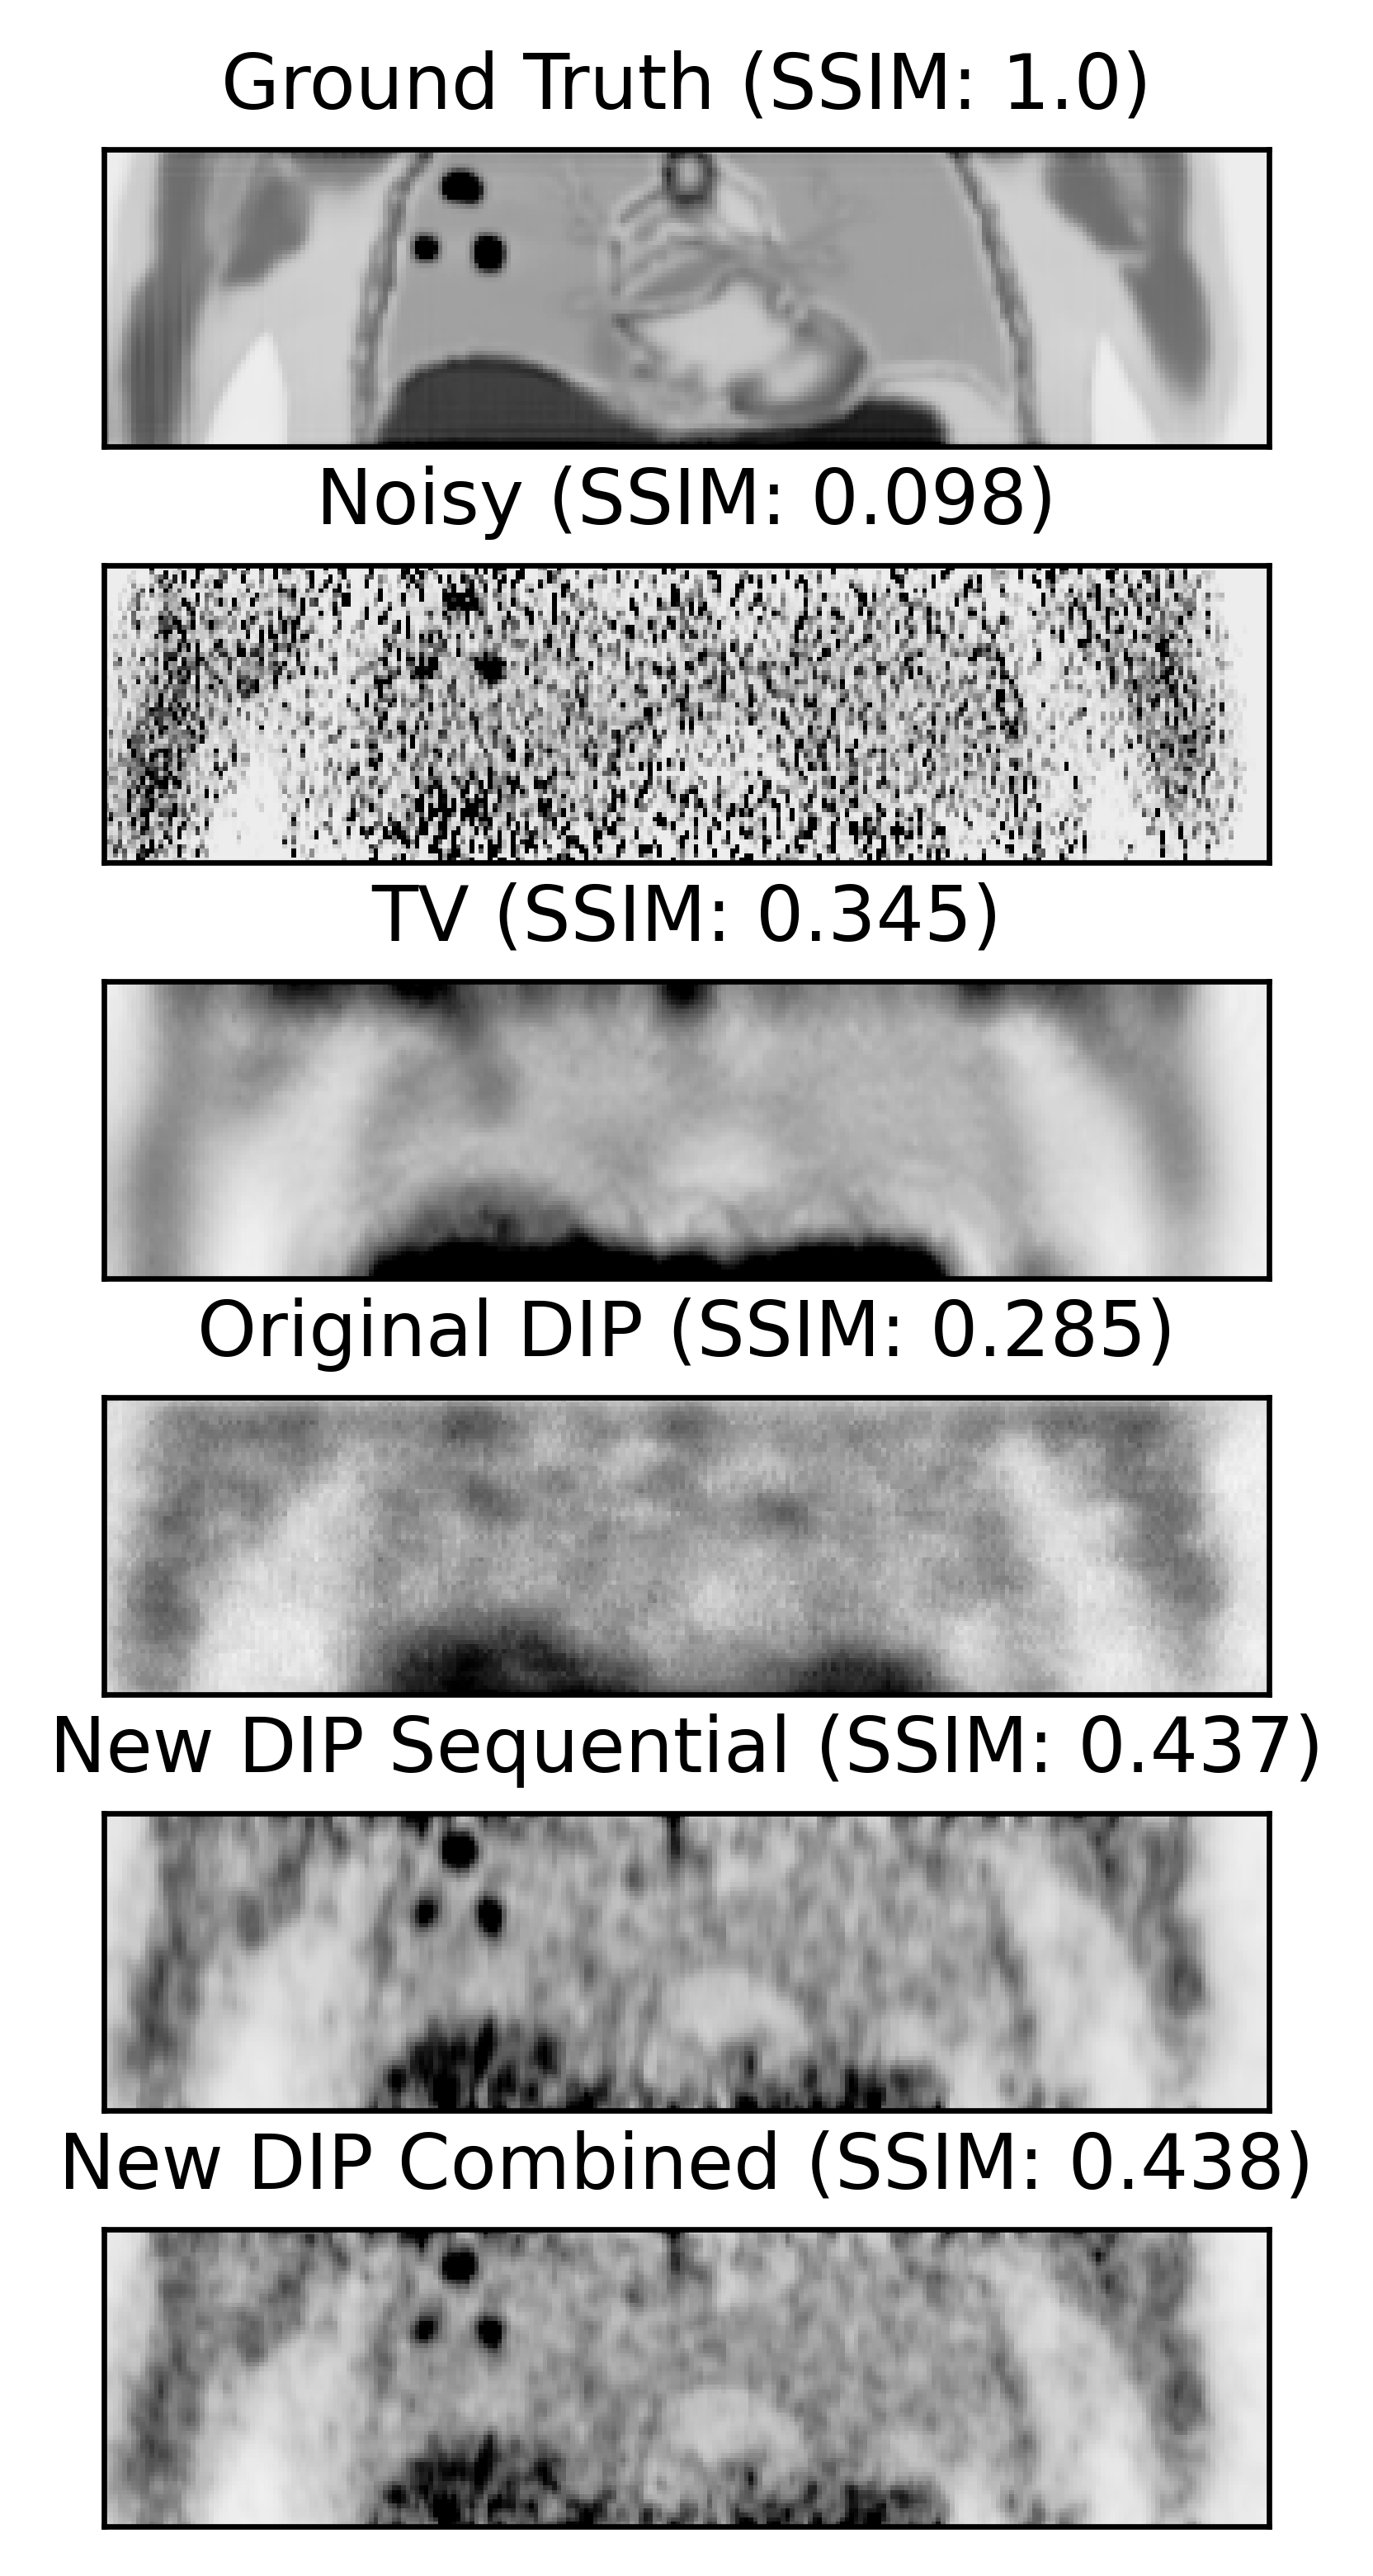
\includegraphics[width=1.0\linewidth]{figures/visual_analysis.png}    
        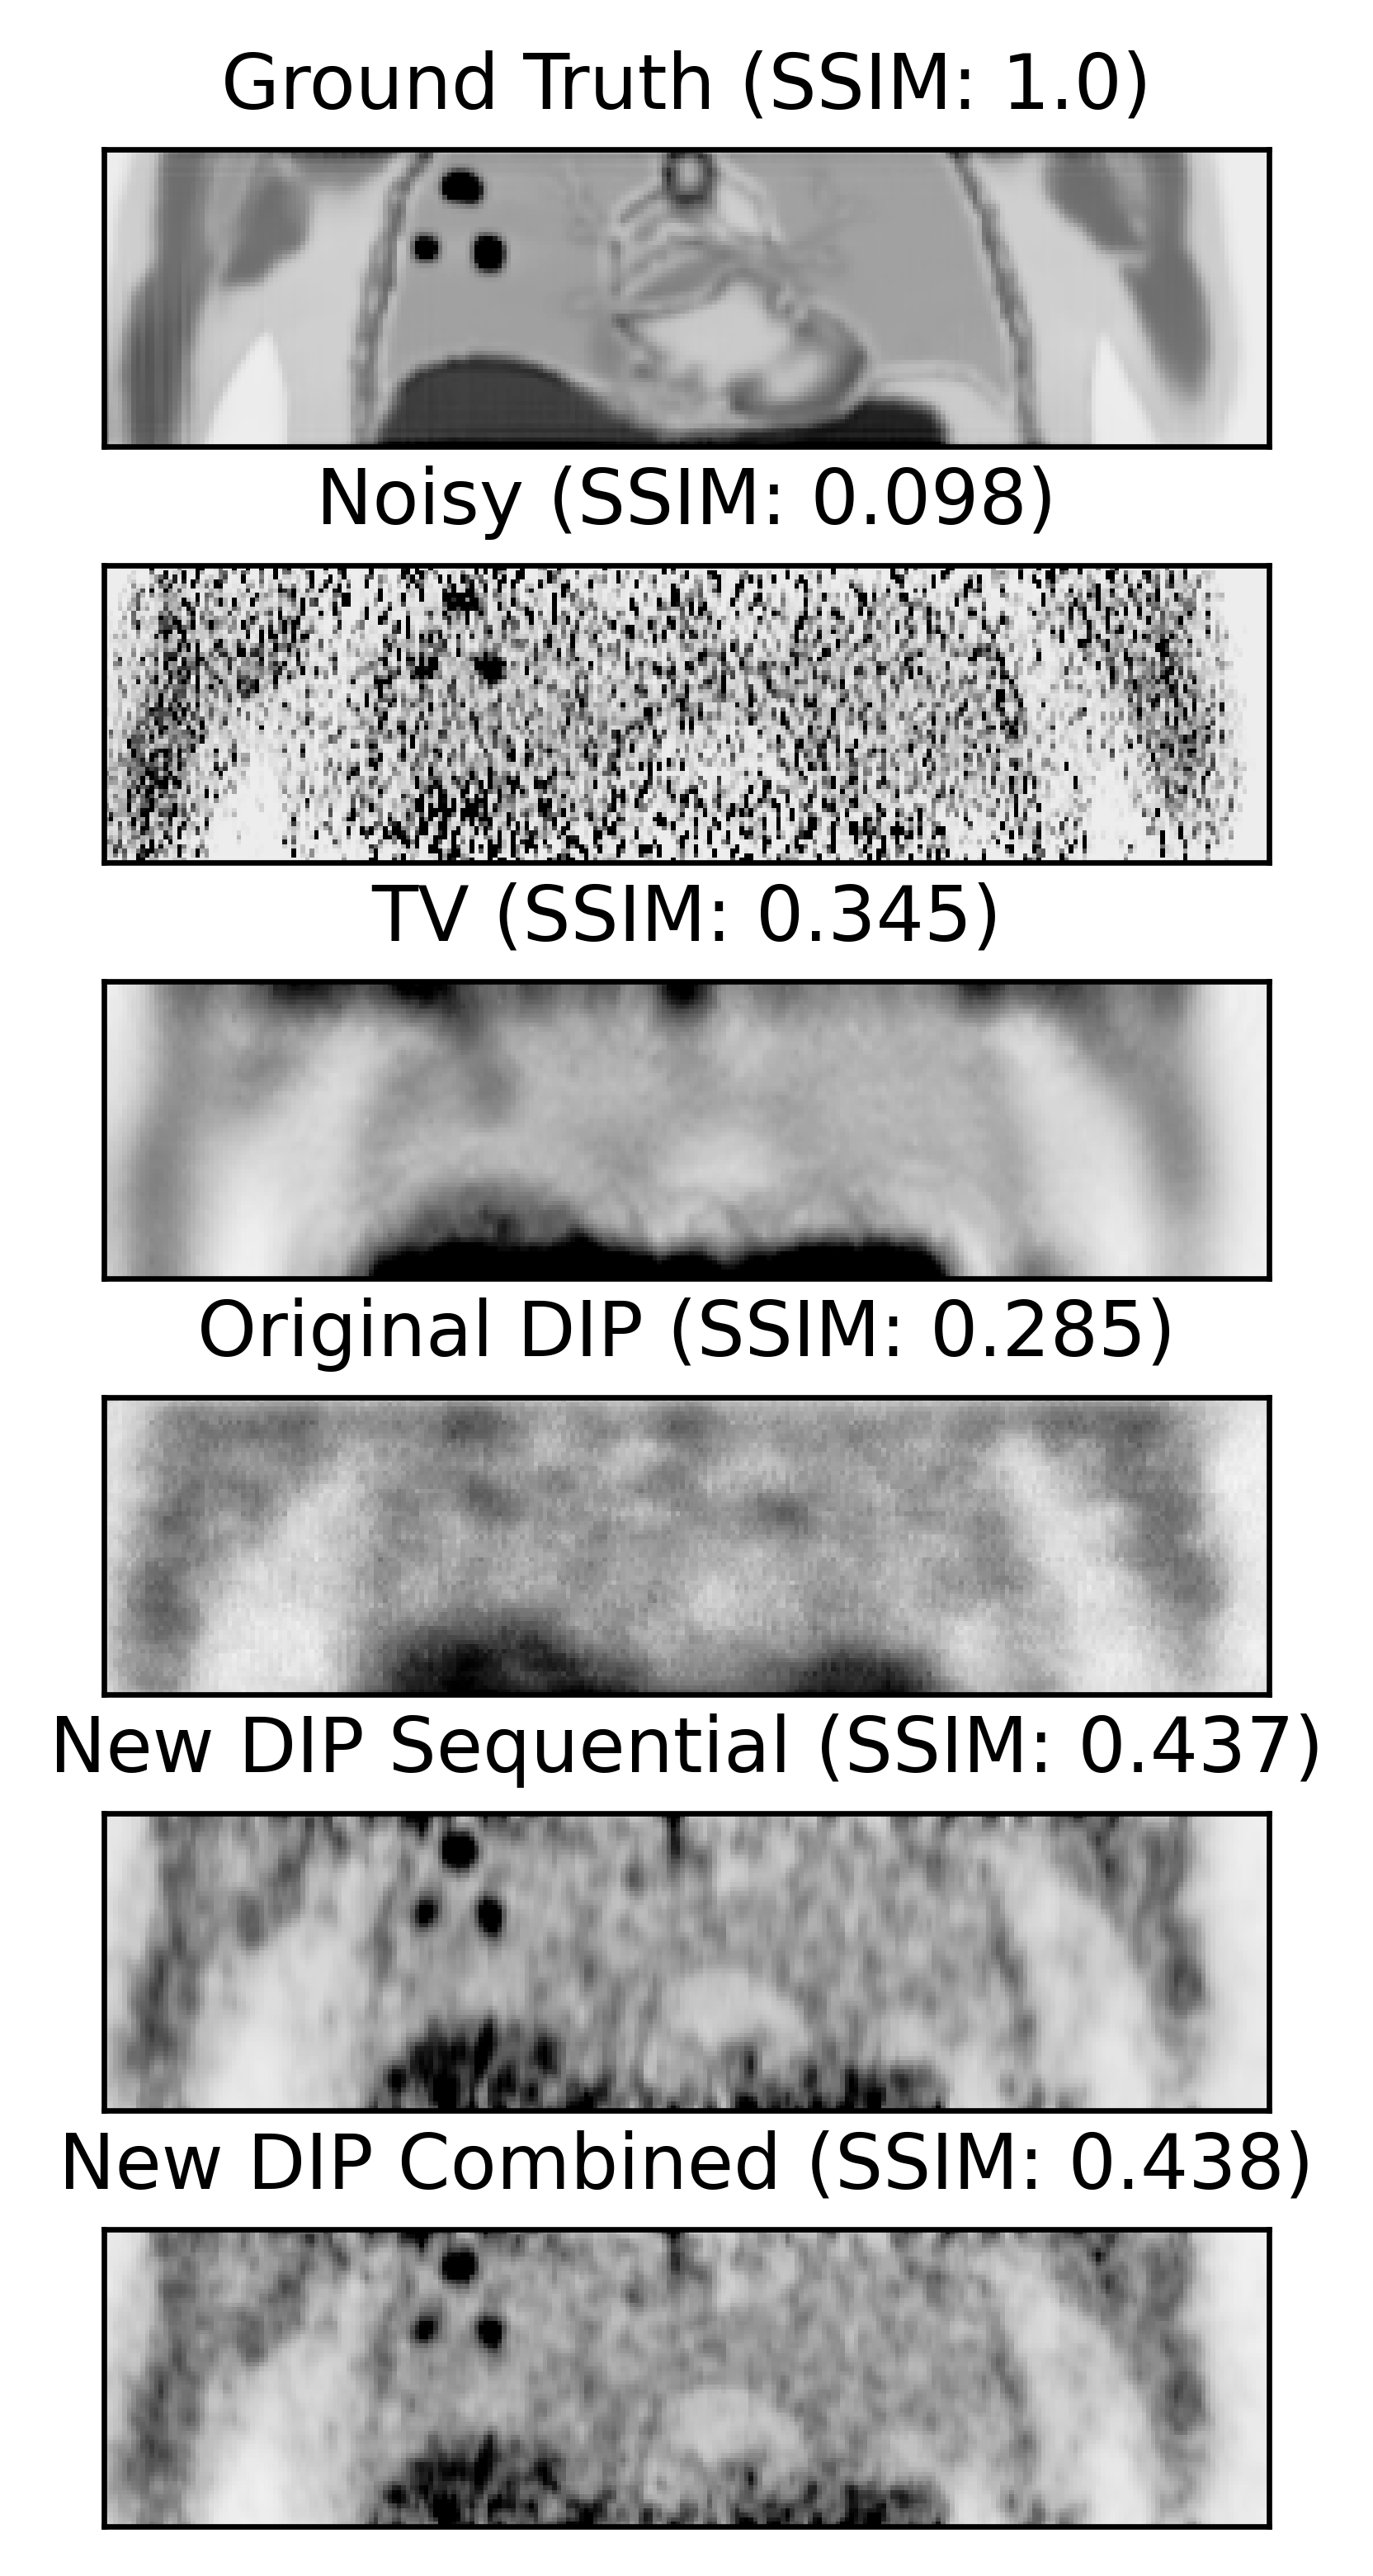
\includegraphics[width=1.0\linewidth]{figures/visual_analysis.png}
        
        % \vspace{-0.5cm}
        
        \captionsetup{singlelinecheck=false, justification=centering}
        \caption{
        % \scriptsize
        First column contains, a visual analysis between the ground truth and denoised results (taken for the last time point, plus \gls{SSIM} to the ground truth), and the second column contains, the $K_i$ results (all voxels in a coronal view) of a Patlak reconstruction of all time points (plus \gls{SSIM} to the ground truth), for; the ground truth, and data denoised using, \gls{TV}, the implementation of \gls{DIP} from~\cite{Gong2019PETPrior}, and our new implementation of \gls{DIP}, trained sequentially and combined (taken for the lung \gls{FOV}). Last row contains, uncertainty volumes, for; the data denoised using our new implementation of \gls{DIP}, trained sequentially and combined (taken for the last time point of the lung \gls{FOV}). Colour map ranges are consistent for all images in each section.}
        
        \label{fig:visual_analysis}
        
        % \vspace{-0.5cm}
    \end{figure}
    
    \begin{figure}
        % \vspace{-0.5cm}
        
        \centering
    
        % 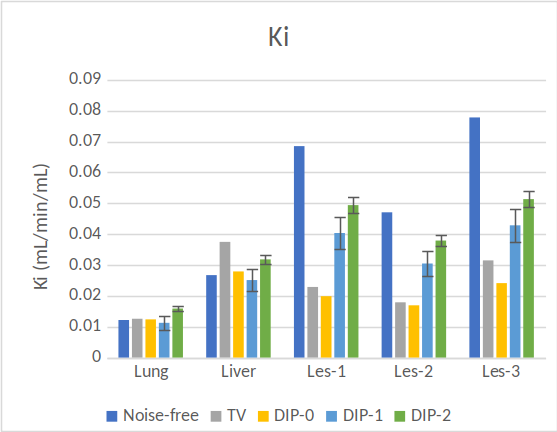
\includegraphics[width=1.0\linewidth]{figures/ki.png}    
        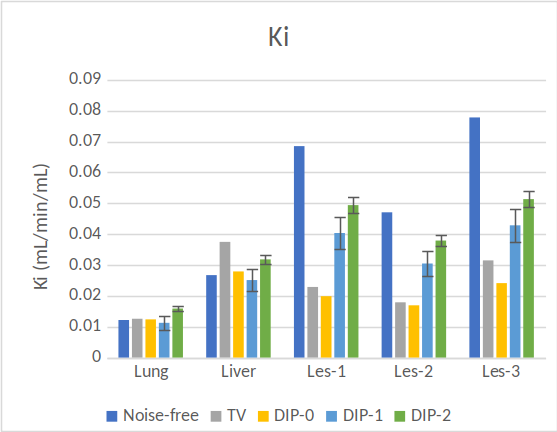
\includegraphics[width=1.0\linewidth]{figures/ki.png}
        
        % \vspace{-0.5cm}
        
        \captionsetup{singlelinecheck=false, justification=centering}
        \caption{
        % \scriptsize
        $K_i$ results (single voxel) of a Patlak reconstruction of all time points, plus uncertainty where applicable, for; the ground truth, and data denoised using, \gls{TV}, the implementation of \gls{DIP} from~\cite{Gong2019PETPrior}, and our new implementation of \gls{DIP}, trained sequentially and combined.}
        
        \label{fig:ki}
        
        % \vspace{-0.5cm}
    \end{figure}
    
    \begin{figure}
        % \vspace{-0.5cm}
        
        \centering
    
        % 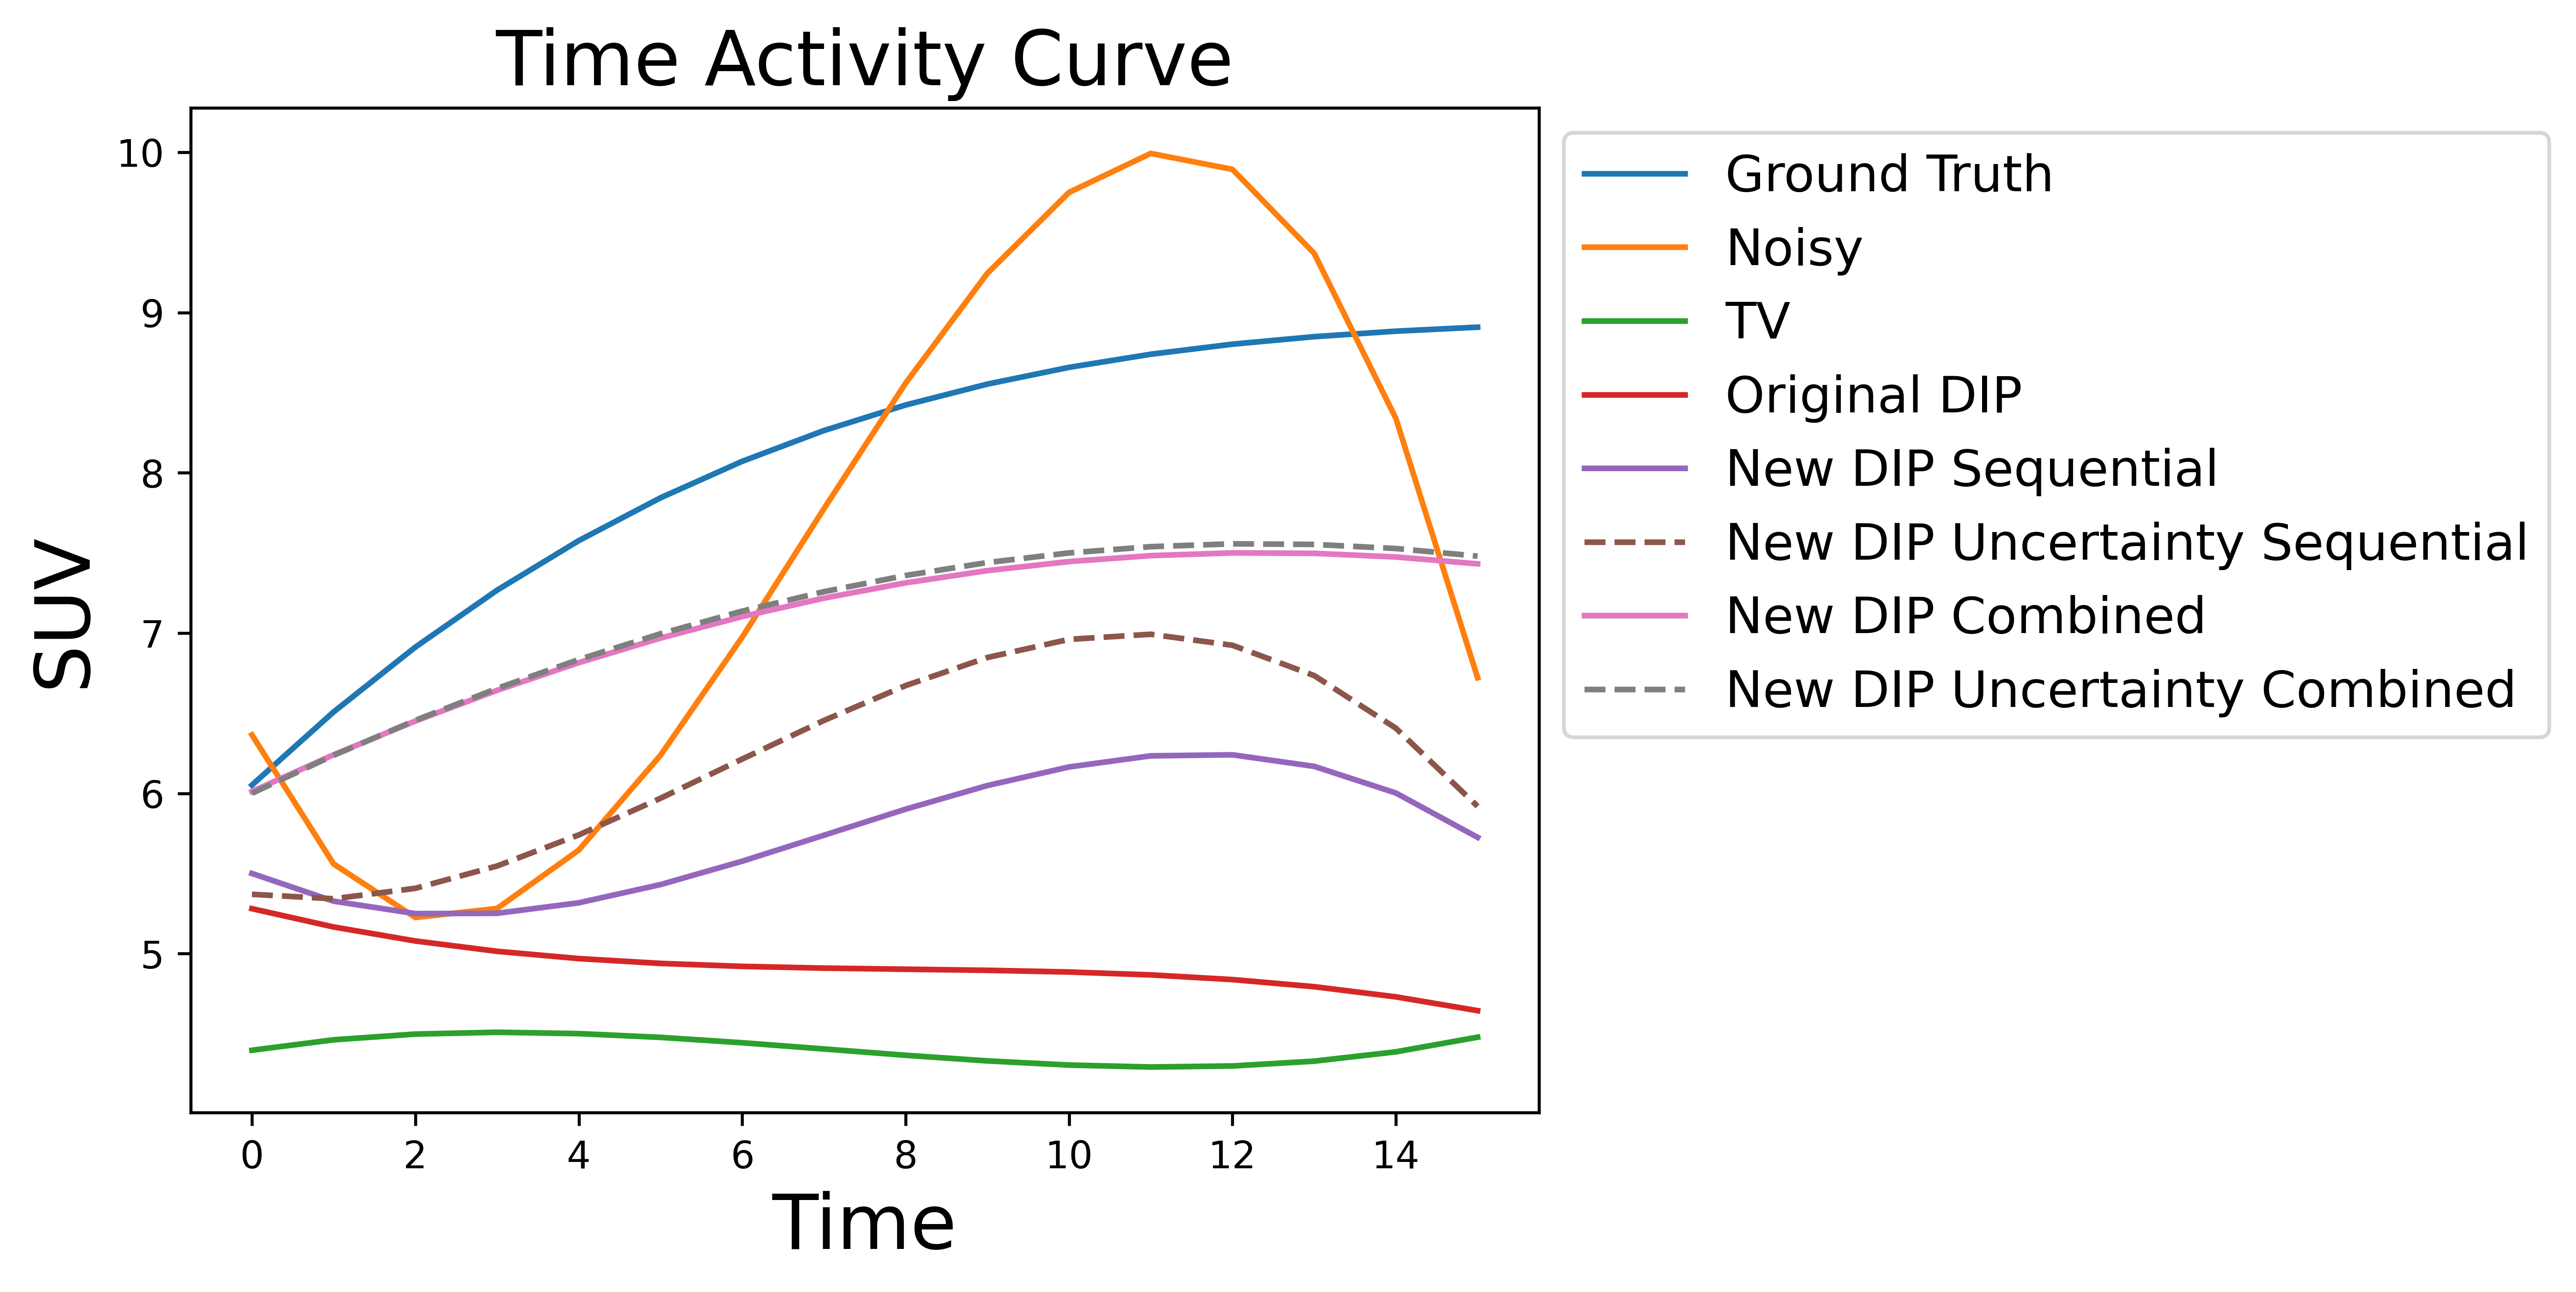
\includegraphics[width=1.0\linewidth]{figures/tac.png}    
        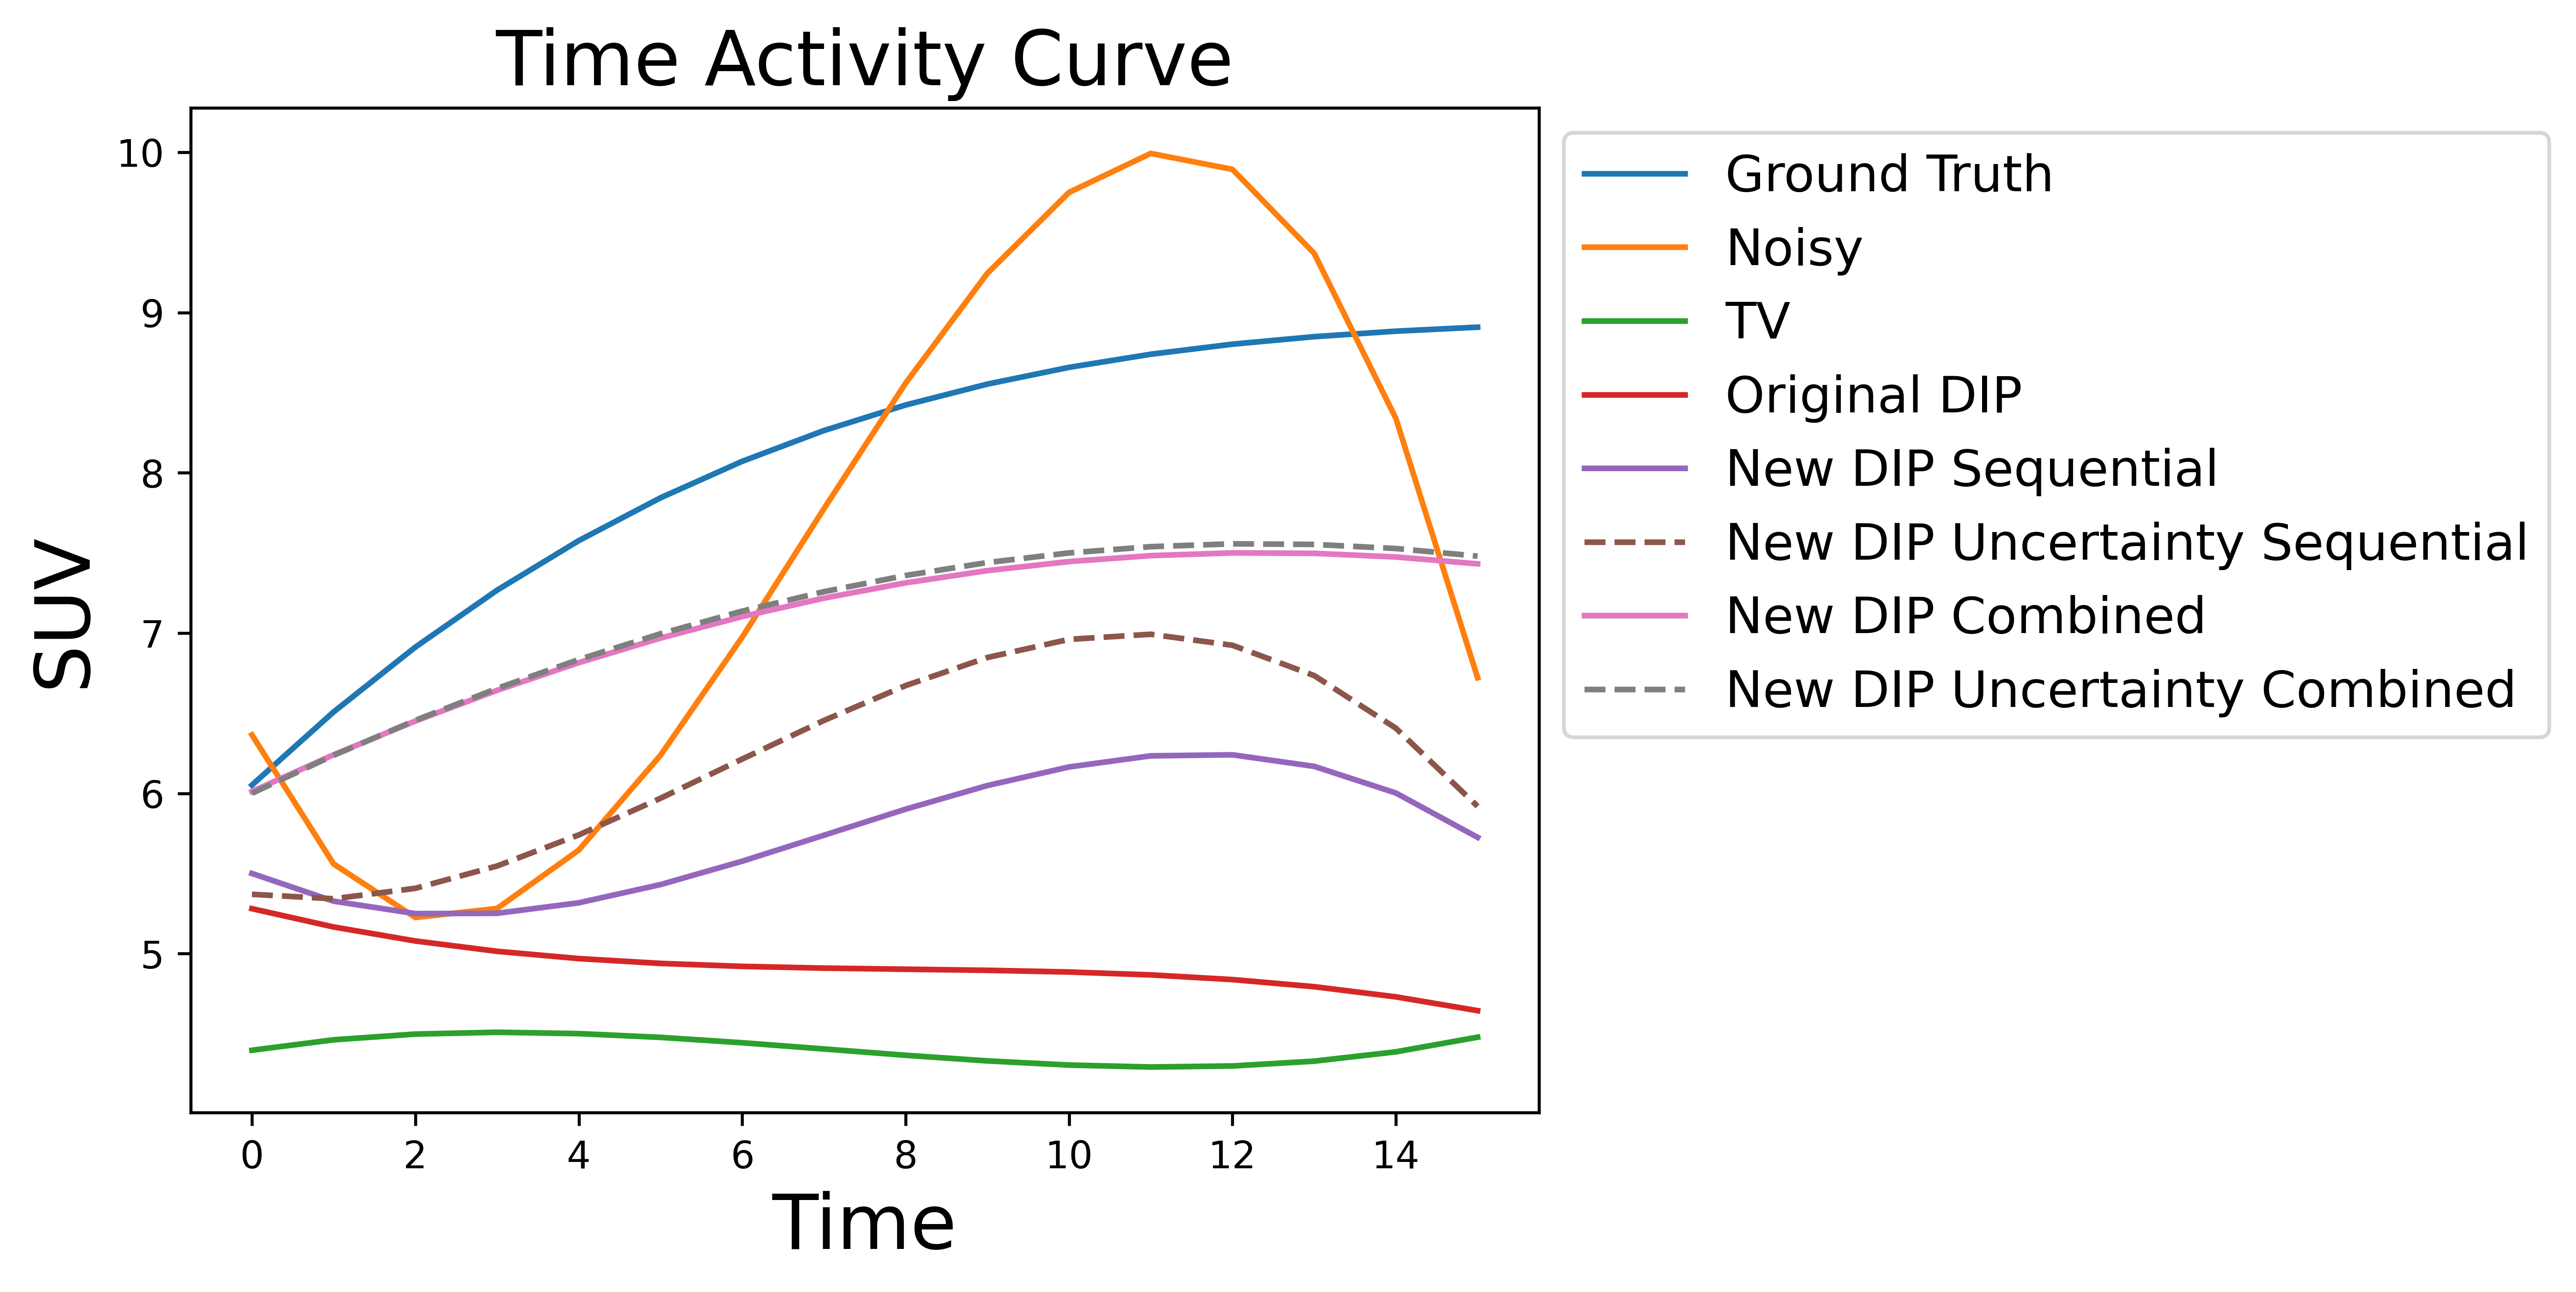
\includegraphics[width=1.0\linewidth]{figures/tac.png}
        
        % \vspace{-0.5cm}
        
        \captionsetup{singlelinecheck=false, justification=centering}
        \caption{
        % \scriptsize
        A \gls{TAC} through a lesion, fit as a third order polynomial regression, with weighting using uncertainty (where available), for; the ground truth, the original noisy data, and this data denoised using, \gls{TV}, the implementation of \gls{DIP} from~\cite{Gong2019PETPrior}, and our new implementation of \gls{DIP}, trained sequentially and combined, both with and without uncertainty (taken for the lung \gls{FOV}).}
        
        \label{fig:tac}
        
        % \vspace{-0.5cm}
    \end{figure}
    
    \begin{figure}
        % \vspace{-0.5cm}
        
        \centering
    
        % 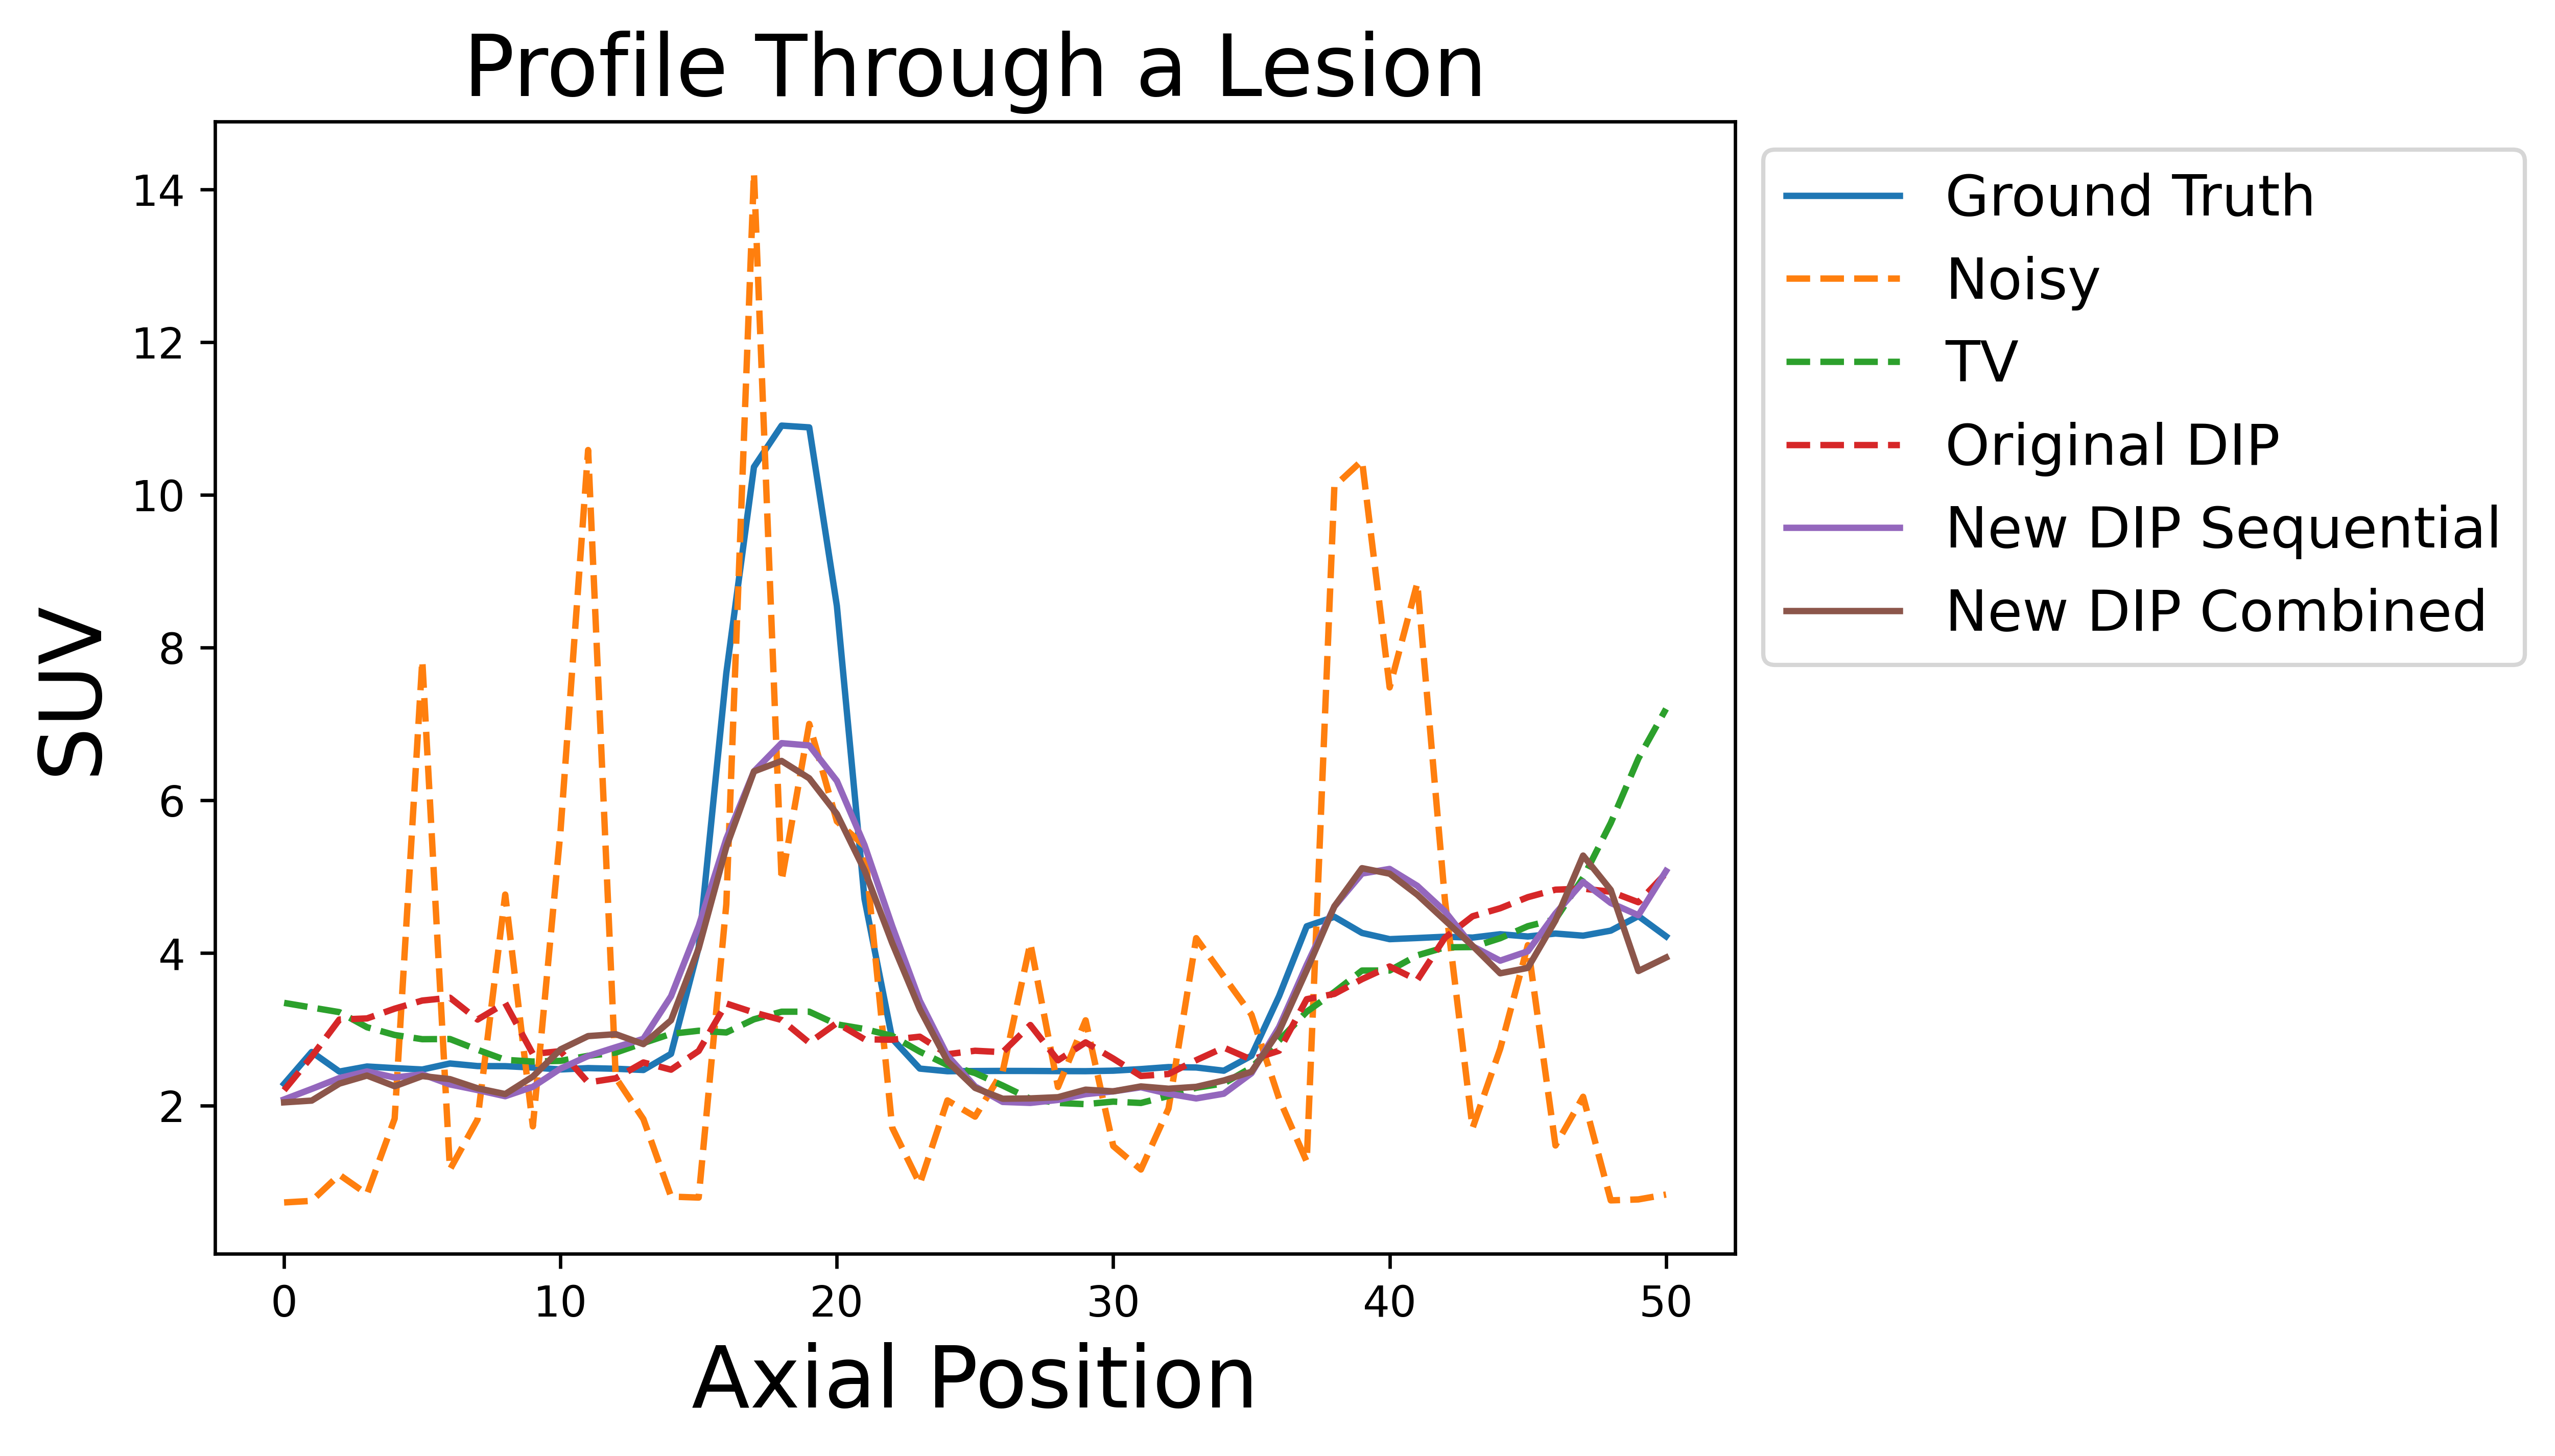
\includegraphics[width=1.0\linewidth]{figures/profile.png}    
        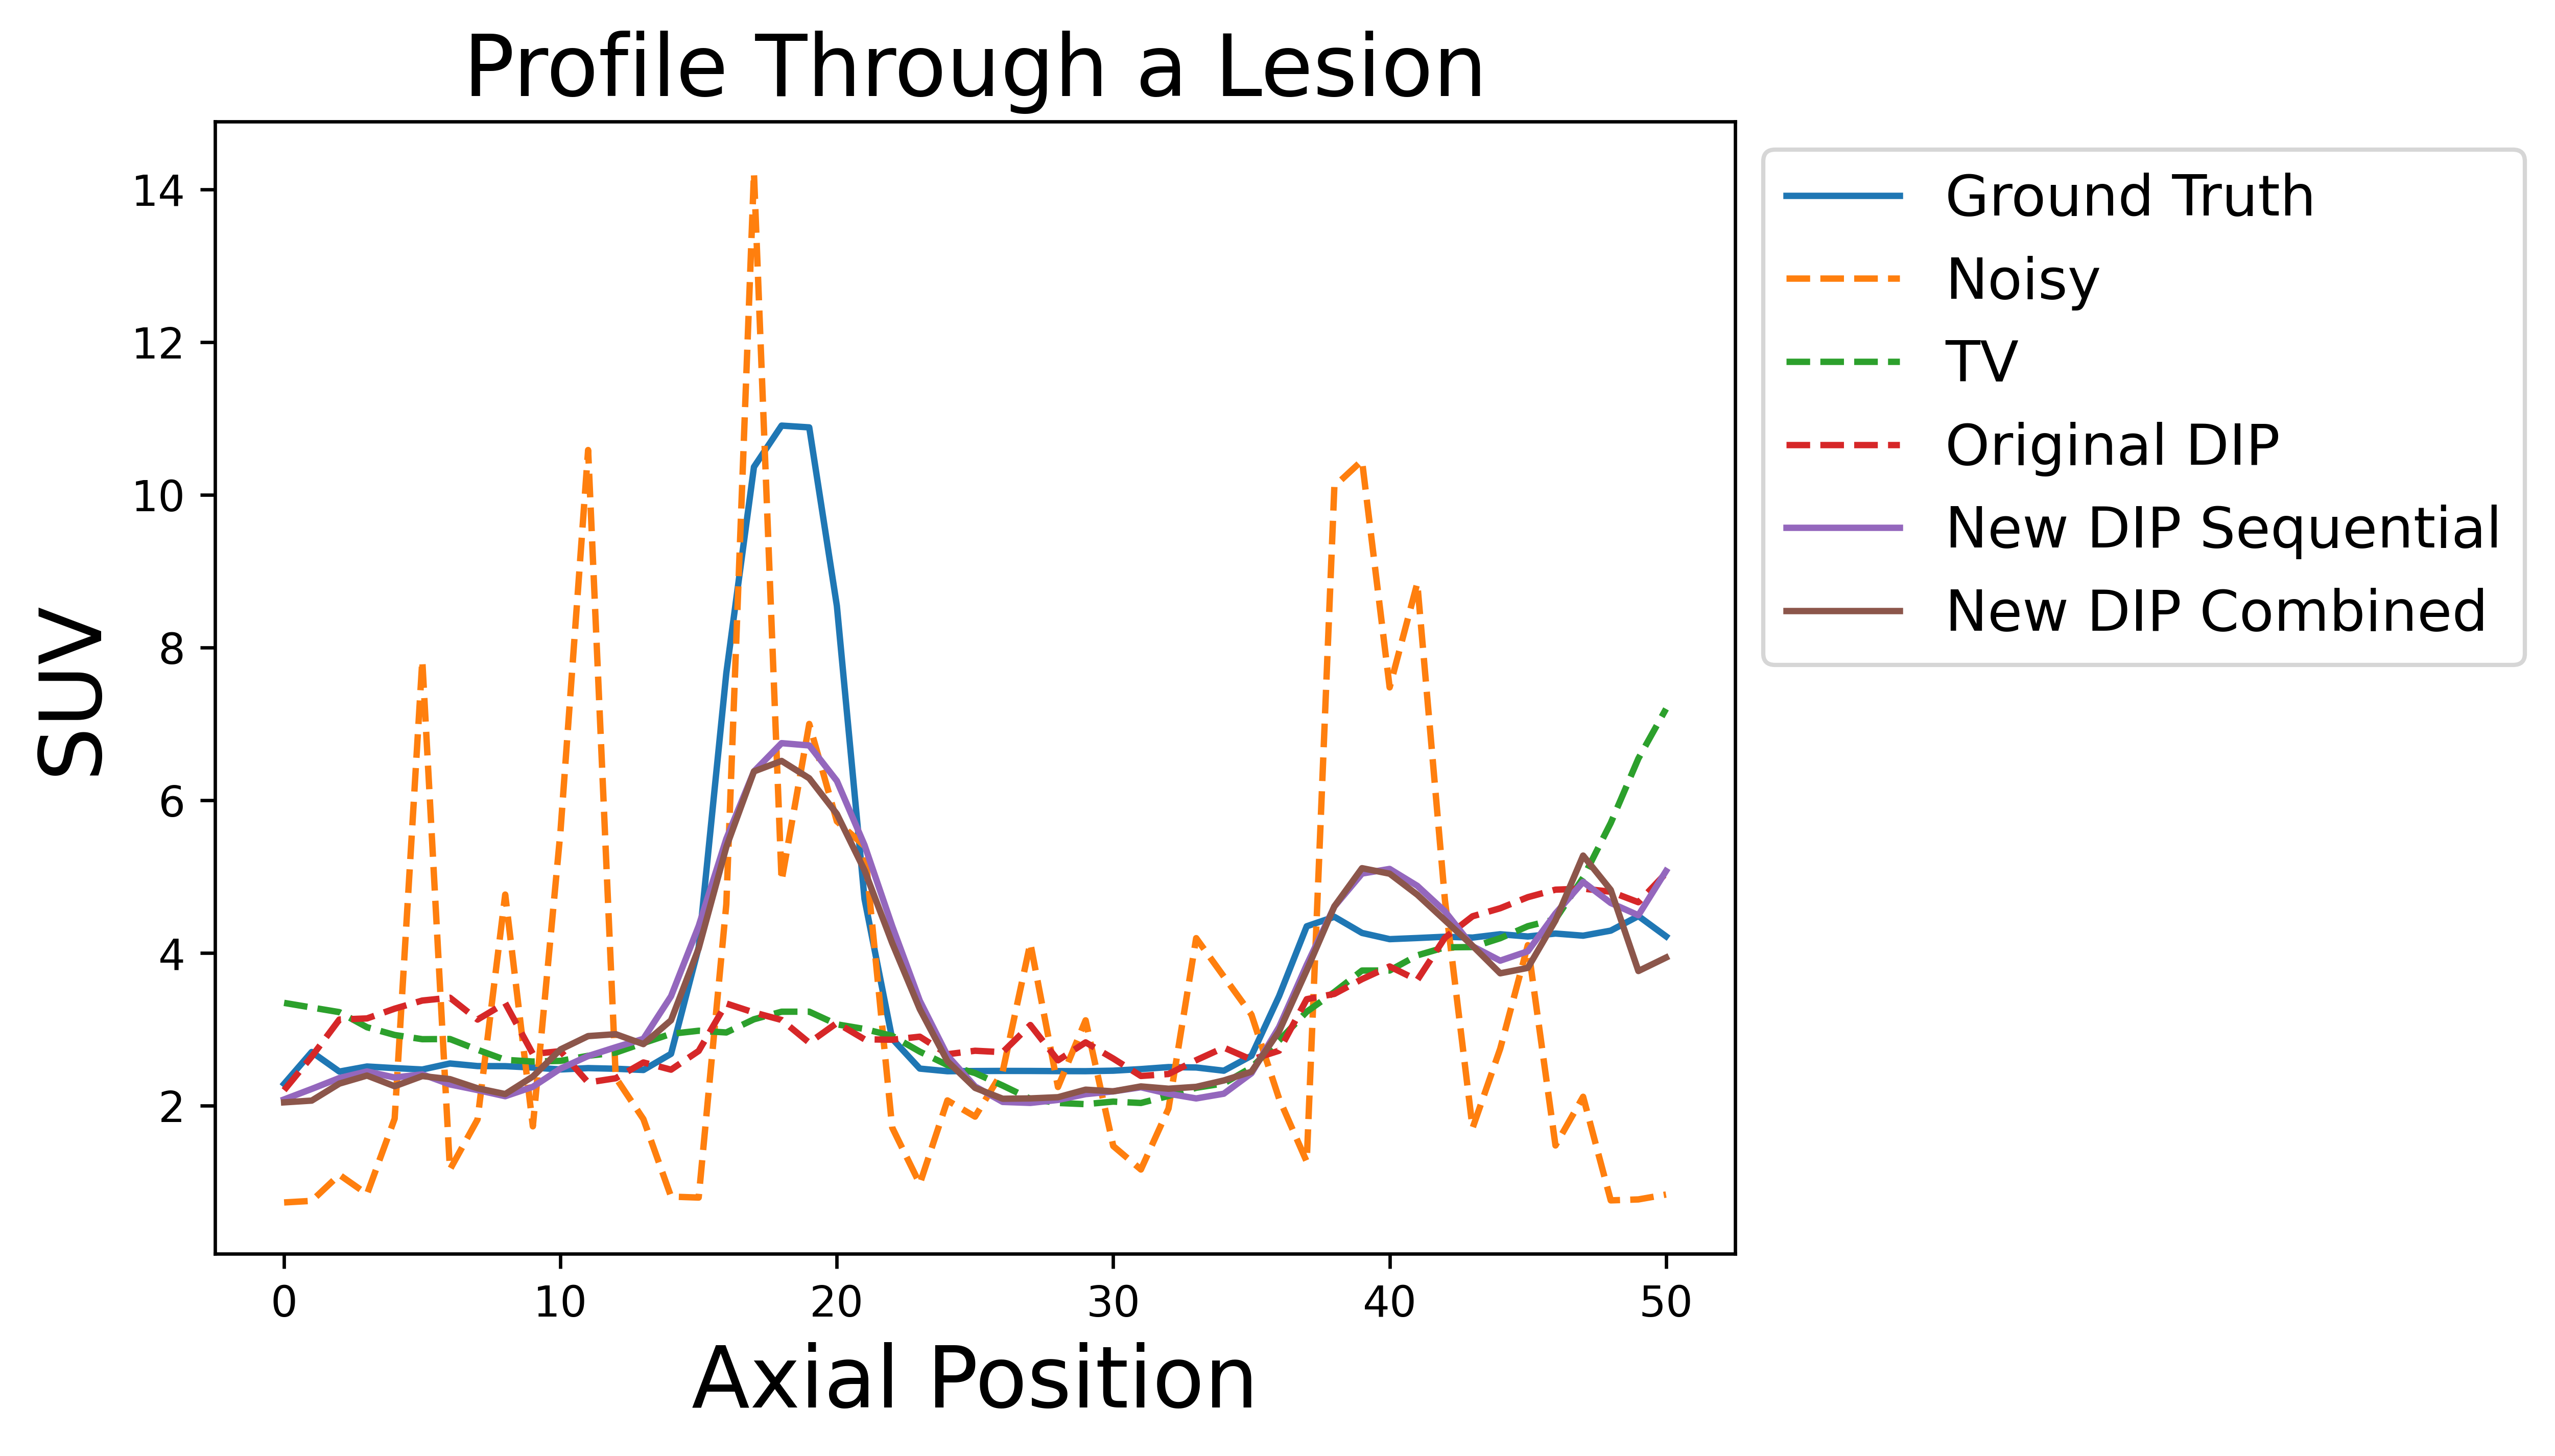
\includegraphics[width=1.0\linewidth]{figures/profile.png}
        
        % \vspace{-0.5cm}
        
        \captionsetup{singlelinecheck=false, justification=centering}
        \caption{
        % \scriptsize
        A profile through a lesion, in the \gls{SI} direction, for; the ground truth, the original noisy data, and this data denoised using, \gls{TV}, the implementation of \gls{DIP} from~\cite{Gong2019PETPrior}, and our new implementation of \gls{DIP}, trained sequentially and combined (taken for the last time point of the lung \gls{FOV}).}
        
        \label{fig:profile}
        
        % \vspace{-0.5cm}
    \end{figure}
    
    \begin{table}
        % \vspace{-0.5cm}
        
        \centering
        
        \captionsetup{singlelinecheck=false, justification=centering}
        \caption{
        % \tiny
        Comparison of \acrshort{SUV}\textsubscript{max} and \acrshort{SUV}\textsubscript{peak}, for; the ground truth, the original noisy data, and this data denoised using, \gls{TV}, the implementation of \gls{DIP} from~\cite{Gong2019PETPrior}, and our new implementation of \gls{DIP}, trained sequentially and combined (taken for the last time point of the lung \gls{FOV}).}
        
        % \vspace{-0.5cm}
        
        % \resizebox*{1.0\linewidth}{!}
        \resizebox*{1.0\linewidth}{!}
        {
            \begin{tabular}{||c|cc||}
                \hline
                \textbf{\acrshort{SUV}}             & \textbf{Max}  & \textbf{Peak} \\
                \hline
                \textbf{Ground Truth}               & $12.3$        & $9.53$ \\
                \hline
                \textbf{Noisy}                      & $21.5$        & $5.99$ \\
                \hline
                \textbf{\gls{TV}}                   & $3.28$        & $6.24$ \\
                \textbf{Original \gls{DIP}}         & $3.90$        & $6.93$ \\
                \hline
                \textbf{New \gls{DIP} Sequential}   & $9.19$        & $8.02$ \\
                \textbf{New \gls{DIP} Combined}     & $9.27$        & $8.21$ \\
                \hline
            \end{tabular}
        }
        \label{tab:suv}
        
        % \vspace{-0.5cm}
    \end{table}
    
    A visual comparison of the reconstructed images (see~\Fref{fig:visual_analysis}), shows that both of the new \gls{DIP} methods perform comparably, if not for a slight reduction in noise in the combined case. Whereas, the \gls{TV} and original \gls{DIP} implementations appear to have struggled with over smoothing, reducing the contrast of the lesions, and introducing some edge artefacts. The uncertainty of the combined method can be seen reduced compared to the sequential method.
    
    A comparison of $K_i$ values across multiple lesions (see~\Fref{fig:ki}), shows that the new \gls{DIP} combined method most often estimates the greatest magnitude of $K_i$ value, which is usually closest to the ground truth. The new \gls{DIP} sequential is slightly less accurate (also with greater uncertainty), however, is more accurate than the \gls{TV} and original \gls{DIP} implementations (which consistently significantly underestimate $K_i$).
    
    The overall shape of the \gls{TAC} (see~\Fref{fig:tac}) for the new \gls{DIP} combined method appears, most similar to the ground truth, however, with a slight reduction in quantification. The sequential method is less accurate, but still more so than both the original \gls{DIP} and \gls{TV} methods. There is significant variation in the noise \gls{TAC}, somewhat masked by the regression, however, its shape is still least like the ground truth. Adding uncertainty appears to have improved the \gls{TAC} of the new \gls{DIP} sequential method, however, the uncertainty of the combined method is less, and as such, the inclusion of uncertainty has not affected results significantly.
    
    The peak of the profile (see~\Fref{fig:profile}) for both new \gls{DIP} methods is comparable, and greater than both the original \gls{DIP} and \gls{TV} methods. The peak of the noise profile is greater than all other methods, including the ground truth, however, this is not necessarily beneficial, as can be seen by the rest of the profile not closely following the ground truth (it undulates unpredictably). The profile for both new \gls{DIP} methods are significantly smoother, and more closely follow the ground truth.
     
    \acrshort{SUV} (and \acrshort{SSIM}) results confirm the above (see~\Fref{tab:suv}).
    % \acrshort{SSIM} results confirm the above.

% \vspace{-0.4cm}

\section{DISCUSSION AND CONCLUSION} \label{sec:discussion_and_conclusion}
    % XXXSome discussion of results here.

    Evaluation indicated that the new \gls{DIP} method, particularly when trained combined, provided images with less noise and more quantitative accuracy than other methods. The combined method had lower uncertainty.

    Results presented here were obtained on a single bed position. Initial evaluation on a bed position, centred on the liver, indicated that parameter fine-tuning, depending on the distribution and count level, will be beneficial. Evaluation with patient data will follow.
    
    The uncertainty estimates produced by the \gls{NN} need to be validated by comparison with results obtained from repeated noise realisations.
    
    % In the future, research will focus on the application of the method to domains other than dynamic \gls{PET}, where \acrshort{4D} data exists, such as \acrlong{MC}.